\section{Using IDL to visualise data}
\label{sec:idl}

  The {\EPOCH} distribution comes with procedures for loading and inspecting
  SDF self-describing data files.
  The IDL routines are held in the {\tt IDL/} directory
  for each of the {\tt epoch*d/} directories. There is also a procedure
  named {\tt Start.pro} in each of the {\tt epoch*d/} directories which is
  used to set up the IDL environment.

  To load data into IDL, navigate to one of the base directories (eg.
  \txt{epoch/trunk/epoch2d/} where \txt{epoch/} is the directory in which you
  have checked out the Subversion repository) and type
  the following:

\begin{boxverbatim}
$> idl Start
IDL Version 7.1.1, Mac OS X (darwin x86_64 m64). (c) 2009, ITT Visual Informat...
Installation number: .
Licensed for use by: STAR404570-32University of Warwick

% Compiled module: SWAPCHR.
% Compiled module: CHECKNAME.
% Compiled module: RETURNIDLUSABLE.
% Compiled module: RETURNFRIENDLYTYPENAME.
% Compiled module: $MAIN$.
% Compiled module: SDFCHECKNAME.
% Compiled module: $MAIN$.
% Compiled module: READVAR.
% Compiled module: LOADCFDFILE.
% Compiled module: HANDLEBLOCK.
% Compiled module: GETMESH.
% Compiled module: GETMESHVAR.
% Compiled module: GETSNAPSHOT.
% Compiled module: READVAR.
% Compiled module: LOADSDFFILE.
% Compiled module: SDFHANDLEBLOCK.
% Compiled module: SDFGETPLAINMESH.
% Compiled module: SDFGETPOINTMESH.
% Compiled module: SDFGETPLAINVAR.
% Compiled module: SDFGETPOINTVAR.
% Compiled module: PARTICLEPHASEPLANE.
% Compiled module: LOADCT.
% Compiled module: FILEPATH.
% LOADCT: Loading table RED TEMPERATURE
% Compiled module: GETDATA.
% LOADCT: Loading table RED TEMPERATURE
IDL> 
\end{boxverbatim}

  This starts up the IDL interpreter and loads in all of the libraries
  for loading and inspecting SDF files.

  We begin by inspecting SDF file contents and finding out what variables
  it contains. To do this we execute the \cmd{list\_variables} procedure call
  which is provided by the {\EPOCH} IDL library.

  At each timestep for which {\EPOCH} is instructed to dump a set of variables a
  new data file is created. These files take the form \txt{0000.sdf}. For
  each new dump the number is incremented.
  The procedure call accepts up to two arguments. The first argument is
  mandatory and specifies the number of the SDF file to be read in.
  This argument can be any integer from 0 to 9999.
  It is padded with zeros and the
  suffix `.sdf' appended to the end to give the name of the data file.
  eg. 99 $\Rightarrow$ `0099.sdf'. The next arguments is optional.
  The keyword \qtt{wkdir} specifies the directory in which the data files
  are located. If this argument is omitted then the currently defined global
  default is used. Initially, this takes the value \qtt{Data} but this can
  be changed using the \cmd{set\_wkdir} procedure and queried using the
  \cmd{get\_wkdir()} function.

\begin{boxverbatim}
IDL> list_variables,0,"Data"
Available elements are
1) Point_electron (Grid) : 2D Point mesh
2) Point_proton (Grid) : 2D Point mesh
3) Grid (Grid) : 2D Plain mesh
4) electron_Weight (Particles) : 1D Point variable
5) proton_Weight (Particles) : 1D Point variable
6) electron_Px (Particles) : 1D Point variable
7) proton_Px (Particles) : 1D Point variable
8) Ex (Electric Field) : 2D Plain variable
9) Ey (Electric Field) : 2D Plain variable
10) Ez (Electric Field) : 2D Plain variable
11) Bx (Magnetic Field) : 2D Plain variable
12) By (Magnetic Field) : 2D Plain variable
13) Bz (Magnetic Field) : 2D Plain variable
14) Jx (Current) : 2D Plain variable
15) Jy (Current) : 2D Plain variable
16) Jz (Current) : 2D Plain variable
17) EkBar (Derived) : 2D Plain variable
18) EkBar_electron (Derived) : 2D Plain variable
19) EkBar_proton (Derived) : 2D Plain variable
20) Number_Density (Derived) : 2D Plain variable
21) en_electron (Grid) : 1D Plain mesh
22) en_electron (dist_fn) : 3D Plain variable
23) Probe_electron_probe (Grid) : 2D Point mesh
24) Px (electron_probe) : 1D Point variable
25) Py (electron_probe) : 1D Point variable
26) Pz (electron_probe) : 1D Point variable
27) weight (electron_probe) : 1D Point variable
IDL>
\end{boxverbatim}

  Each variable in the SDF self-describing file format is assigned a
  name and a class as well as being defined by a given variable type.
  The \cmd{list\_variables} procedure prints out the variable name followed
  by the variable's class in parenthesis. Following the colon is a
  description of the variable type.

  To retrieve the data, you must use the \cmd{getdata()} function call.
  The function must be passed a snapshot number, either as the first argument
  or as a keyword parameter \qtt{snapshot}. It also accepts the wkdir as
  either the second argument or the keyword parameter \qtt{wkdir}. If it is
  omitted alltogether, the current global default is used. Finally, it accepts
  a list of variables or class of variables to load.
  Since it is a function, the result must be assigned to a
  variable. The object returned is an IDL data structure containing a list
  of named variables.

  To load either a specific variable or a class of variables, specify the
  name prefixed by a forward slash. It should be noted here that the IDL
  scripting language is not case sensitive so $P_x$ can be specified as
  either \qtt{/Px} or \qtt{/px}.

  We will now load and inspect the \qtt{Grid} class, this time omitting
  the optional \qtt{wkdir} parameter. This time we will load from the
  third dump file generated by the {\EPOCH} run, which is found in the
  file \txt{0002.sdf} since the dump files are numbered starting from zero.
%
\pagebreak
\subsection{Inspecting Data}

\begin{boxverbatim}
IDL> gridclass = getdata(1,/grid)

IDL> help,gridclass,/structures
** Structure <1a800008>, 10 tags, length=268513928, data length=268513920, refs=1:
   FILENAME        STRING    'Data/0001.sdf'
   TIMESTEP        LONG                42
   TIME            DOUBLE       5.0109036e-15
   GRID_ELECTRON   STRUCT    -> <Anonymous> Array[1]
   GRID_PROTON     STRUCT    -> <Anonymous> Array[1]
   GRID            STRUCT    -> <Anonymous> Array[1]
   X               DOUBLE    Array[1024]
   Y               DOUBLE    Array[512]
   GRID_EN_ELECTRON
                   STRUCT    -> <Anonymous> Array[1]
   ELECTRON_PROBE  STRUCT    -> <Anonymous> Array[1]

IDL> help,gridclass.grid,/structures
** Structure <1529cf8>, 5 tags, length=12376, data length=12376, refs=2:
   X               DOUBLE    Array[1025]
   Y               DOUBLE    Array[513]
   LABELS          STRING    Array[2]
   UNITS           STRING    Array[2]
   NPTS            LONG      Array[2]
\end{boxverbatim}

  Here we have used IDL's built in \qtt{help} routine and passed the
  \qtt{/structures} keyword which prints information about a structure's
  contents rather than just the structure itself.

  Since \qtt{Grid} is a class name, all variables of that class have
  been loaded into the returned data structure. It is a nested type
  so many of the variables returned are structures themselves and those
  variables may contain structures of their own.

  The \qtt{Grid} variable itself contains \qtt{x} and \qtt{y} arrays
  containing the $x$ and $y$ coordinates of the 2D cartesian grid. The
  other variables in the \qtt{Grid} structure are metadata used to identify
  the type and properties of the variable.
  In order to access the \qtt{Grid} variable contained within the
  \qtt{gridclass} data structure we have used the \qtt{.} operator.
  In a similar way, we would access the \qtt{x} array contained within
  the \qtt{Grid} variable using the identifier \qtt{gridclass.grid.x}.

\subsection{Getting Help in IDL}
  IDL is a fairly sophisticated scripting environment with a large
  library of tools for manipulating data. Fortunately, it comes with a
  fairly comprehensive array of documentation. This can be accessed by
  typing \cmd{?} at the IDL prompt.

\begin{boxverbatim}
IDL> ?
% ONLINE_HELP: Starting the online help browser.
IDL>
\end{boxverbatim}
  \begin{center}
    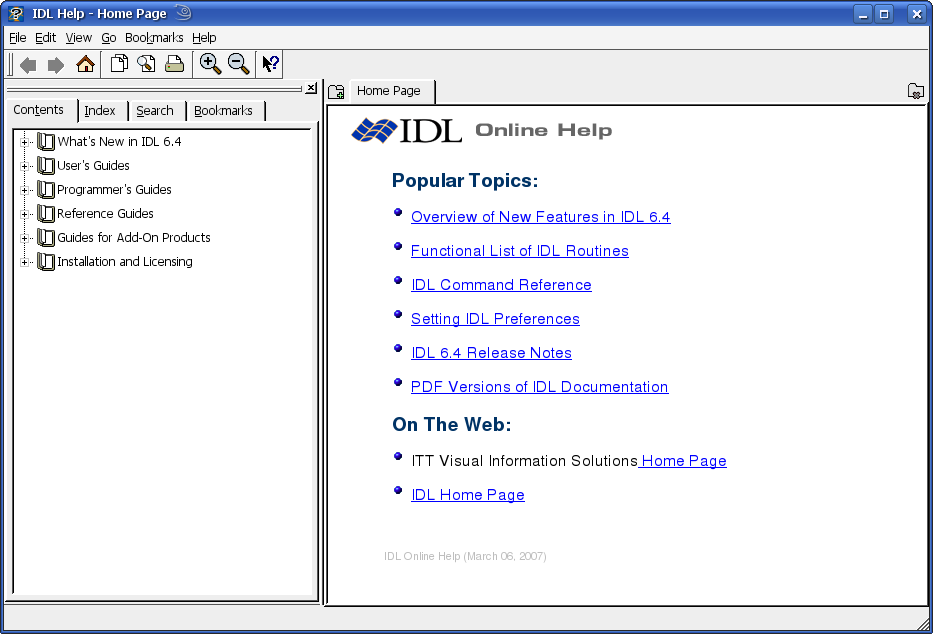
\includegraphics[width=0.8\linewidth]{images/idl_help}
  \end{center}

  The documentation is divided into books aimed at users or developers and
  is fully searchable and cross indexed.

\subsection{Manipulating And Plotting Data}
  Once the data has been loaded from the SDF file we will want to extract
  the specific data we wish to analyse, perhaps perform some mathematical
  operations on it and then plot the results.

  To do this we must learn a few basic essentials about the IDL scripting
  language. Since we are all familiar with the basic concepts shared by
  all computer programming languages, I will just provide a brief overview
  of the essentials and leave other details to the excellent on-line
  documentation.

  IDL supports multidimensional arrays similar to those found in the
  FORTRAN programming language. Whole array operations are supported
  such as \qtt{5*array} to multiply every element of \qtt{array} by $5$.
  Also matrix operations such as addition and multiplication are supported.

  The preferred method for indexing arrays is to use brackets. It is
  possible to use parenthesis instead but this usage is deprecated.
  Column ordering is the same as that used by FORTRAN, so to access
  the $(i,j,k)$th element of an array you would use \qtt{array[i,j,k]}.
  IDL arrays also support ranges so \qtt{array[5:10,3,4]} will return
  a one dimensional array with five elements. \qtt{array[5:*]} specifies
  elements five to $n$ of an $n$ element array. \qtt{array[*,3]} picks
  out the third row of an array.

  There are also a wide range of routines for querying and transforming
  arrays of data. For example, finding minimum and maximum values,
  performing FFTs, etc. These details can all be found by searching the
  on-line documentation. 

  Finally, IDL is a full programming language so you can write your own
  functions and procedures for processing the data to suit your needs.

\subsection{1D Plotting in IDL}
  The most commonly performed plot and perhaps the most useful data analysis
  tool is the 1D plot. In IDL, this is performed by issuing the command
  \cmd{plot,x,y} where \qtt{x} and \qtt{y} are one dimensional arrays of
  equal length. For each element \qtt{x[i]} plotted on the $x$-axis the
  corresponding value \qtt{y[i]} is plotted along the $y$-axis. As a
  simple example:
\begin{boxverbatim}
IDL> plot,[1,2,3],[2,2,5]
\end{boxverbatim}
  Gives rise to the following plot:
  \begin{center}
    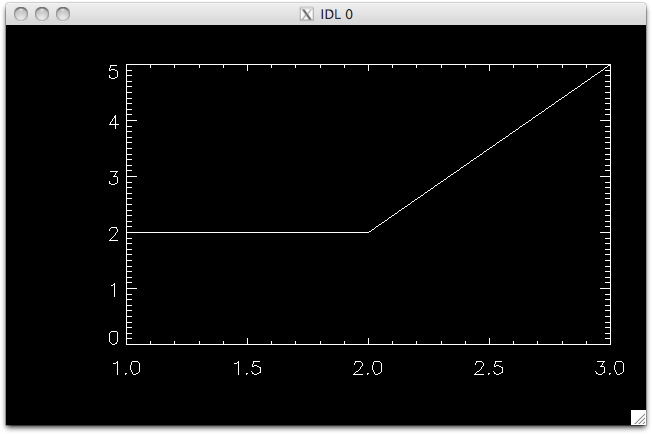
\includegraphics[width=0.7\linewidth]{images/idl_simple_plot}
  \end{center}

  As a more concrete example, we will now take a one-dimensional slice through
  the 2D\linebreak \qtt{Number\_Density} array read in from our SDF data file.
  In this example we will give the $x$ and $y$ axes labels by passing extra
  parameters to the \qtt{plot} routine. A full list of parameters can be found
  in the on-line documentation. In this example we also make use of the
  \qtt{\$} symbol which is IDL's line continuation character.

\begin{boxverbatim}
IDL> data = getdata(0)
IDL> plot,data.x,data.number_density[*,256],xtitle='x', $
IDL>    ytitle='number density'
\end{boxverbatim}
  This command generates the following plot:
  \begin{center}
    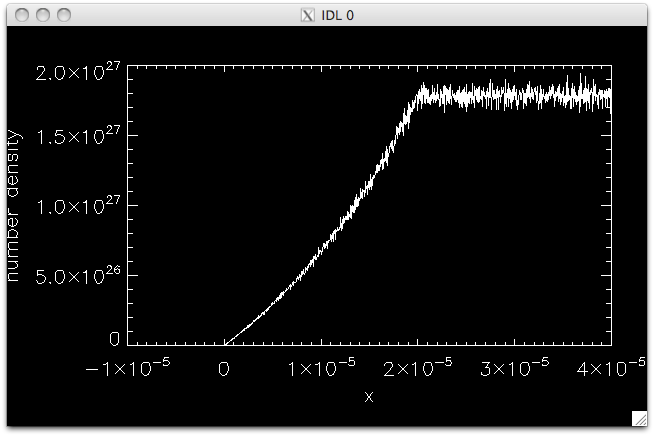
\includegraphics[width=0.7\linewidth]{images/idl_plot}
  \end{center}

\subsection{Postscript Plots}
  The plots shown so far have just been screen-shots of the interactive
  IDL plotting window. These are fairly low quality and could included as
  figures in a paper.

  In order to generate publication quality plots, we must output to the
  postscript device. IDL maintains a graphics context which is set using
  the \cmd{set\_plot} command. The two most commonly used output devices
  are \qtt{x} which denotes the X-server and \qtt{ps} which is the postscript
  device. Once the desired device has been selected, various attributes
  of its behaviour can be altered using the \cmd{device} procedure.
  For example, we can set the output file to use for the postscript plot.
  By default, a file with the name \qtt{idl.ps} is used.

  Note that this file is not fully written until the postscript device is
  closed using the \cmd{device,/close} command. When we have finished our
  plot we can resume plotting to screen by setting the device back to \qtt{x}.

\begin{boxverbatim}
IDL> set_plot,'ps'
IDL> device,filename='out.ps'
IDL> plot,data.x,data.number_density[*,256],xtitle='x', $
IDL>    ytitle='number density',charsize=1.5
IDL> device,/close
IDL> set_plot,'x'
\end{boxverbatim}

  This set of commands results in the following plot being written to
  a file named \qtt{out.ps}.
  \begin{center}
    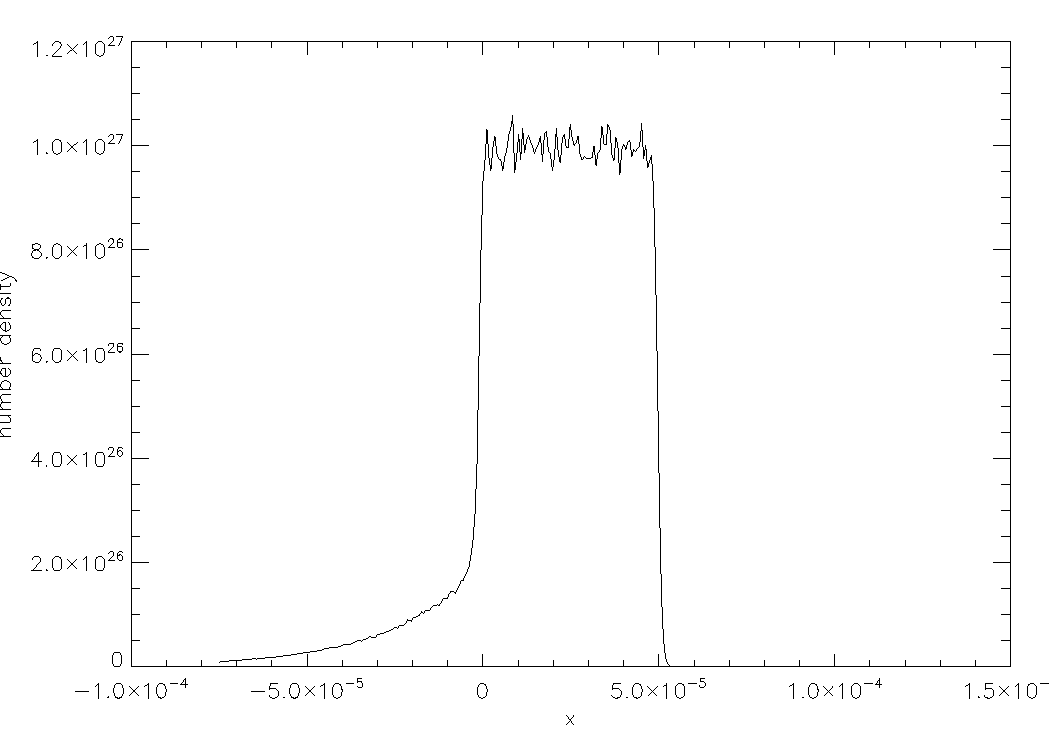
\includegraphics[width=0.8\linewidth]{images/idl_ps_plot}
  \end{center}
  By default, IDL draws its own set of fonts called ``Hershey vector fonts".
  Much better looking results can be obtained by using a postscript font
  instead. These options are passed as parameters to the \cmd{device}
  procedure. More details can be found in the on-line documentation under
  ``Reference Guides $\Rightarrow$ IDL Reference Guide $\Rightarrow$
  Appendices $\Rightarrow$ Fonts".

\subsection{Contour Plots in IDL}
  Whilst 1D plots are excellent tools for quantitive analysis of data,
  we can often get a better qualitative overview of the data using 2D
  or 3D plots.

  One commonly used plot for 2D is the contour plot. The aptly named
  \cmd{contour,z,x,y} procedure takes a 2D array of data values, \qtt{z},
  and plots them against $x$ and $y$ axes which are specified in the
  1D \qtt{x} and \qtt{y} arrays. The number of contour lines to plot is
  specified by the \qtt{nlevels} parameter. If the \qtt{/fill} parameter
  is used then IDL will fill each contour level with a solid colour rather
  than just drawing a line at the contour value.

  The example given below plots a huge number of levels so that a smooth
  looking plot is produced. \qtt{xstyle=1} requests that the $x$ axes drawn
  exactly matches the data in the \qtt{x} variable rather than just using
  a nearby rounded value and similarly for \qtt{ystyle=1}.
\begin{boxverbatim}
IDL> n=100
IDL> levels=max(data.number_density)*findgen(n)/(n-1)
IDL> colors=253.*findgen(n)/(n-1)+1
IDL> contour,data.number_density,data.x,data.y,xstyle=1,ystyle=1, $
IDL>    levels=levels,/fill,c_colors=colors 
\end{boxverbatim}
  Issuing these commands gives us the contour plot shown below. Note that
  the colour table used is not the default one but has been constructed to
  be similar to the one used by VisIt.
  \begin{center}
    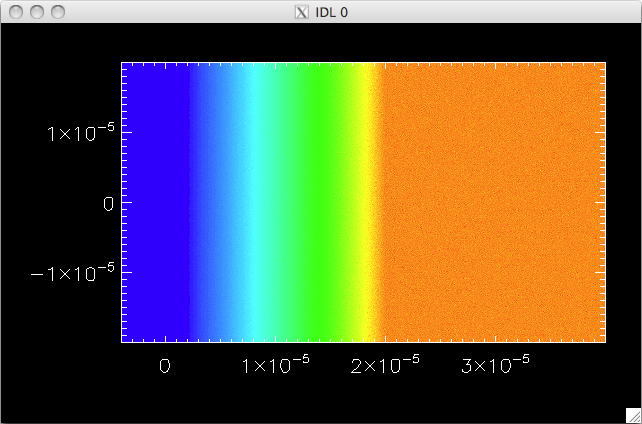
\includegraphics[width=0.8\linewidth]{images/idl_contour}
  \end{center}


\subsection{Shaded Surface Plots in IDL}
  Another method for visualising 2D datasets is to produce a 3D plot in
  which the data is elevated in the $z$ direction by a height proportional
  to its value. IDL has two versions of the surface plot. \cmd{surface}
  produces a wireframe plot and \cmd{shade\_surf} produces a filled and
  shaded one. As we can see from the following example, many of IDL's
  plotting routines accept the same parameters and keywords.

  The first command shown here, \cmd{loadct,3}, asks IDL to load the third
  colour table which is\linebreak ``RED\_TEMPERATURE".

\begin{boxverbatim}
IDL> loadct,3
IDL> shade_surf,data.number_density,data.x,data.y,xstyle=1, $
IDL>    ystyle=1,xtitle='x',ytitle='y',ztitle='number density',charsize=3
\end{boxverbatim}
  \begin{center}
    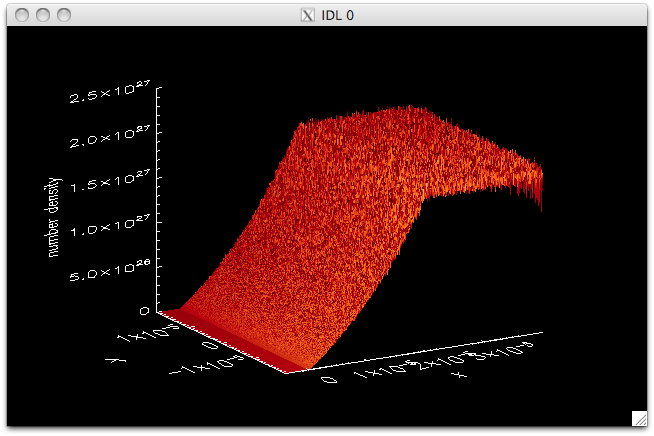
\includegraphics[width=0.8\linewidth]{images/idl_shade_surf}
  \end{center}

\subsection{Interactive Plotting}
  Finally, in recent versions of IDL it is now possible to perform all of
  these plot types in an interactive graphical user interface. The corresponding
  procedures are launched with the commands \cmd{iplot}, \cmd{icontour}
  and \cmd{isurface}.

\begin{boxverbatim}
IDL> iplot,data.x,data.number_density[*,256]
\end{boxverbatim}
  \begin{center}
    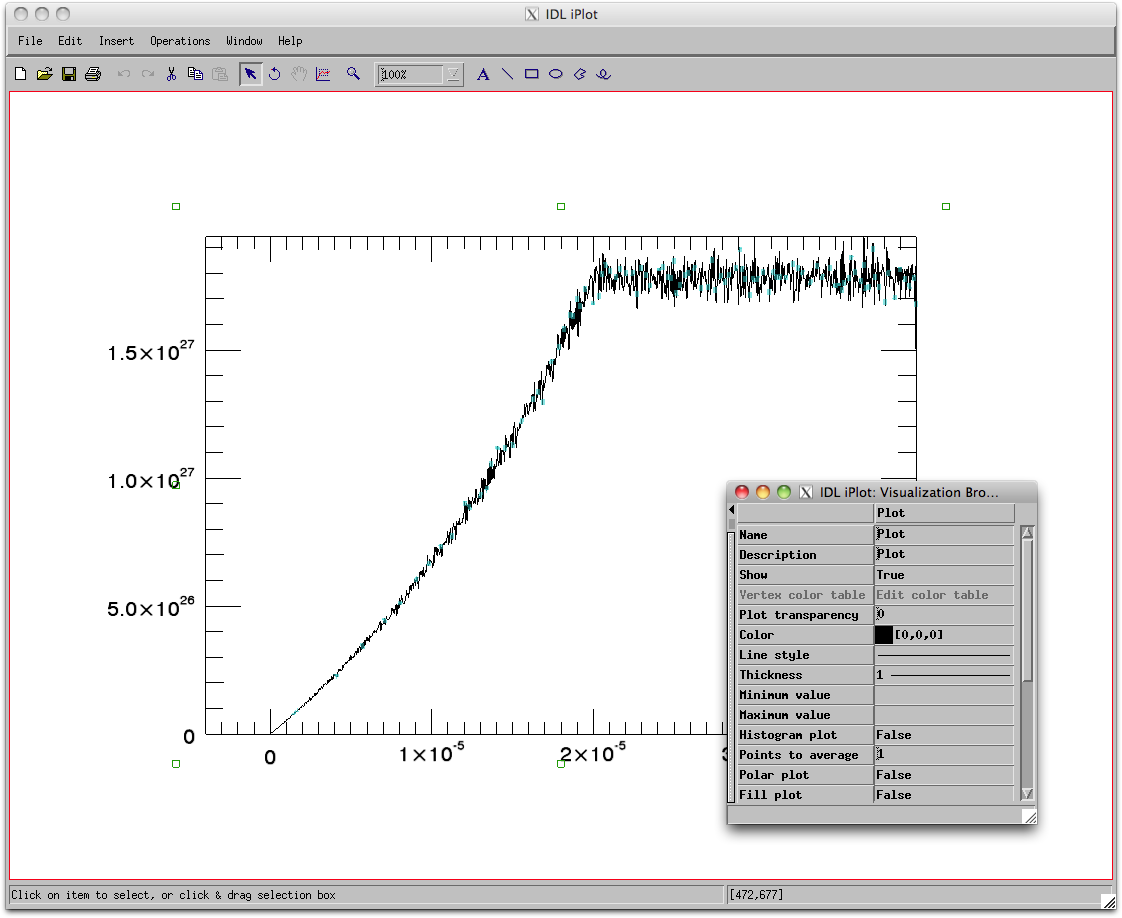
\includegraphics[width=0.8\linewidth]{images/idl_iplot}
  \end{center}

  IDL is an extremely useful tool but it also comes with a fairly hefty
  price tag. If you are not part of an organisation that will buy it for
  you then you may wish to look into a free alternative. It is also a
  proprietary tool and you may not wish to work within the restrictions
  that this imposes.

  There are a number of free tools available which offer similar functionality
  to that of IDL, occasionally producing superior results.

  For a simple drop-in replacement, the GDL project aims to be fully compatible
  and works with the existing {\EPOCH} IDL libraries after a couple of small
  changes. Other tools worth investigating are {\em ``yorick"} and
  {\em ``python"} with the {\em ``SciPy"} libraries. At present there is
  no SDF reader for either of these utilities but one may be developed if
  there is sufficient demand.

\section{Using VisIt to visualise data}

\subsection{LLNL VisIt}
LLNL's VisIt software is a parallel data visualisation package
(\inlinecode{https://wci.llnl.gov/codes/visit/}). {\EPOCH} comes with source
code for the plug-in needed to allow VisIt to load the SDF output files which
are generated by {\EPOCH}. There are full manuals for VisIt which can be
downloaded from the above link so no further details will be given here. To
build the plug-in, first ensure that the visit binary is in the \$PATH
environment variable. Then simply type ``make visit'' in one of the
\inlinecode{epoch\{1,2,3\}d} directories.
For more experienced
users of VisIt, the xml file which is used to generate the plug-in is supplied
in the VisIt subdirectory, called \inlinecode{SDF2.xml}.

  Whilst IDL is an excellent tool for visualising 1D and 2D datasets, it
  is extremely poor when it comes to dealing with 3D data. For this purpose,
  we recommend the use of the {\em ``VisIt"} visualisation tool.

  The other great advantage that VisIt has over IDL is the ability to
  render in parallel, enabling the visualisation of huge datasets which
  IDL would be incapable of dealing with.

  \begin{itemize}
  \item
    Initially developed by the Department of Energy (DOE) Advanced Simulation
    and Computing Initiative (ASCI) 
  \item
    Now developed and maintained by the Lawrence Livermore National Laboratory
    along with a group of external contributors
  \item
    Written in C++ and supports python and Java interfaces
  \item
    Available for UNIX (Irix, Tru64, AIX, Linux, Solaris), Mac OS X
    (10.3 - 10.9), and Windows platforms
  \item
    Open source and freely available under the BSD license
  \item
    Plots, operators and database readers are implemented as plugins allowing
    the VisIt to be dynamically extended at run-time
  \item
    Powerful set of tools for manipulating, analysing and visualising 3D
    datasets
  \item
    Parallel and distributed architecture for visualising huge data sets
  \end{itemize}

\subsection{Obtaining And Installing VisIt}
  Both the source code and pre-compiled binaries are available for download
  from the projects web page which is found at the URL
  {\tt https://wci.llnl.gov/codes/visit/home.html}

  \begin{center}
    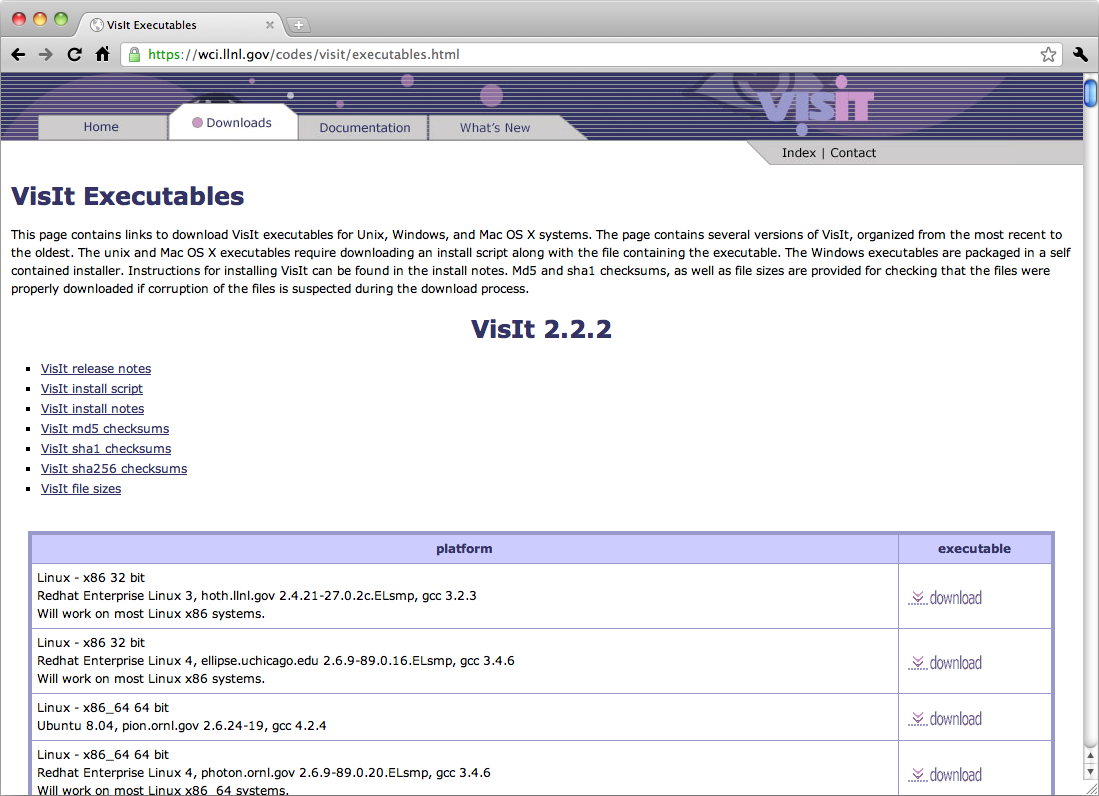
\includegraphics[width=0.8\linewidth]{images/visit_web}
  \end{center}

  There are full instructions for compiling the project from source code
  along with build scripts written to help ease the process. However, this
  is not recommended as it is an extremely large tool and the compilation
  takes hours to complete. It is usually far easier to download a pre-compiled
  binary which matches your system architecture.

  However, occasionally compilation may be a necessary step. Linux
  in particular is a moving target and it is not always possible to
  find a binary which matches the particular combination of libraries
  installed on your system.

  The easiest way to install the VisIt tool is to ask the system
  administrator to do it for you. However, this may not always be the
  best option. The system in question may be run by someone who is
  not concerned with your particular software needs or has insufficient
  skills to deal with the task. In any case, VisIt has a fairly rapid
  release schedule and you may find that some functionality you need
  is not present in the version installed on the machine.

  Fortunately, for all these scenarios it is usually quite easy to install
  a copy in your own home directory. Just find a binary on the web page
  {\tt https://wci.llnl.gov/codes/visit/executables.html} which closely
  matches your machine and download it. This can be unpacked into your
  home directory with the command
  \cmd{tar xzf visit2\_2\_2.linux-x86\_64.tar.gz}. The actual name of
  the file will vary depending on which version you downloaded. This
  will unpack the VisIt binary into a subdirectory named \txt{visit/}.
  Now all that is necessary is to add this to your search path.
  eg. \cmd{export PATH=\$HOME/visit/bin:\$PATH}

  These instructions illustrate the steps required for installing your
  own copy of VisIt when you have no other choice. VisIt is an extremely
  large program, so if a version is already available then it is usually
  better to use the installed version.

  The machines at Warwick have a recent version of VisIt installed which
  is available via the \qtt{modules} system. To make use of it you must
  first issue the command \cmd{module load visit}.

\subsection{Compiling The Reader Plugin}

  One piece of compilation which is almost always necessary is that of
  the SDF reader plugin. This is shipped as source code in a subdirectory
  of the {\EPOCH} repository. It is located in the \txt{VisIt/} subdirectory
  of the main \txt{epoch/} directory. The reader will work for any
  SDF file generated by any code which uses the SDF I/O routines. You do
  not need a separate reader for each version of {\EPOCH}.

  To compile, first navigate to one of the \txt{epoch*d/} directories in your
  {\EPOCH} repository. Just type ``make visit'' and the build scripts should
  take care of the rest.
  The SDF reader plugin will be installed into the directory
  \txt{\$HOME/.visit/linux-intel/plugins/databases/} on your system.
  Note that the \txt{linux-intel/} component will vary depending on
  your machine operating system and architecture.

  Each time you install a new version of VisIt you must recompile the reader
  to match the new installation. It will also occasionally be necessary to
  recompile when changes occur to the SDF data format or the reader plugin
  itself. The developers will notify users if this is the case, although
  it does no harm to regularly recompile the reader as a matter of course.

  We will see later that it is possible to do remote data visualisation
  with VisIt in which the GUI is launched and interacted with on one
  machine and the data files are located on a separate machine entirely.
  In this situation the reader must be installed on the remote machine and
  must match the setup there. The setup on the local machine is unimportant.
  In fact it is not even necessary to have the plugin installed on the
  local machine. This is particularly useful when using a Windows environment
  to analyse data located on a remote UNIX workstation.

\subsection{Loading Data Into VisIt}
  \begin{center}
    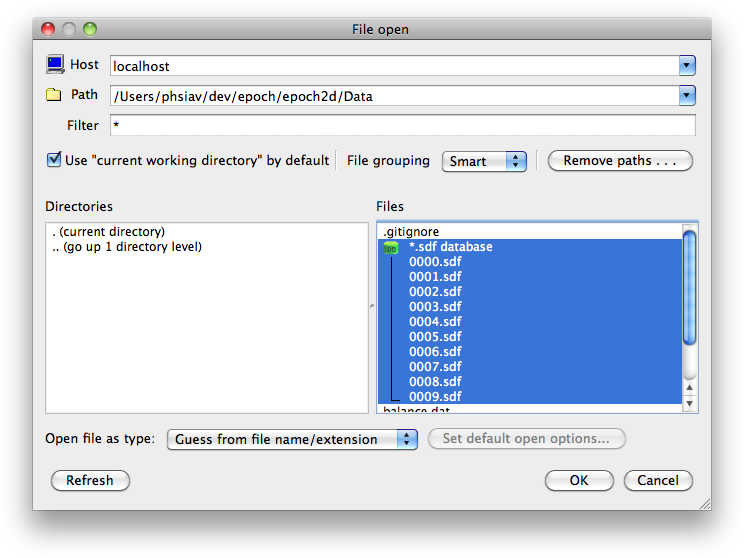
\includegraphics[width=0.8\textwidth]{images/visit_db_list}
  \end{center}

  The most straightforward method for loading data into VisIt is to
  start the application and then browse the filesystem for the dataset
  you are interested in. This is done by selecting \qm{File $\Rightarrow$
  Open file} from the VisIt menu bar. A file selection dialogue will appear
  allowing you to browse directories along with the options to filter
  the results according to a given regular expression and grouping options.
  By default, VisIt will attempt to group all files containing the same
  suffix and some kind of numbering system into a sort of virtual database.

  The right-hand pane of this window shows a list of selected files which
  will appear in the main VisIt window when you are finished.

  An alternative method of specifying the data file to open is to pass
  a command line option when the tool is launched. An example of this
  method is \cmd{visit -o Data/0000.sdf}. When the file is specified in
  this manner the list of files shown in the VisIt window will also
  include the full list of files in the dataset's subdirectory and
  all the files in the current working directory. The other SDF files
  will be grouped together in a virtual database.

  Yet another method for selecting the dataset to use is by opening a
  previously saved session file. Will discuss this further in a later section

  \begin{center}
    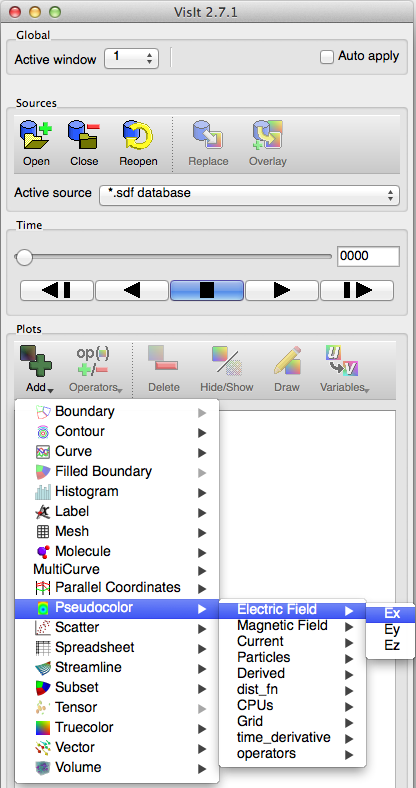
\includegraphics[height=0.7\textheight]{images/visit_select_var}
  \end{center}
  Once a SDF file has been successfully loaded the \qm{Add} menu item
  will become un-greyed and the cycle numbers for each file in the virtual
  database will be displayed. If we navigate to one of the plot types we
  are able to select the variable to plot from a drop-down list.

\subsection{Contour Plots in VisIt}
  We will now replicate each of the plots which we generated using IDL
  in earlier sections. For reasons which will soon become clear we begin
  with the contour plot and move on to the 1D plot in the next section.

  Having opened the same dataset we were using in the IDL discussion we
  now select the \qm{Add} menu item. Notice that many of the plot
  types listed here are greyed out and cannot be selected. This is because
  many of the plots are dependent on the type or dimensionality of the
  variable to be plotted. If our dataset contains no variables which match
  the required properties for a plot, the plot menu will be disabled.

  For the current dataset there is no \qm{Boundary} plot available since this
  requires multi-material data and none of our variables meet
  that criteria.

  The list contains a menu item for a \qm{Contour} plot. We are not going
  to select this item since it only generates a contour plot with lines
  indicating each contour level and not a filled version. Instead we
  choose \qm{Add $\Rightarrow$ Pseudocolor $\Rightarrow$ Derived $\Rightarrow$
  Number\_Density} and then hit the \qm{Draw} button.
  \begin{center}
    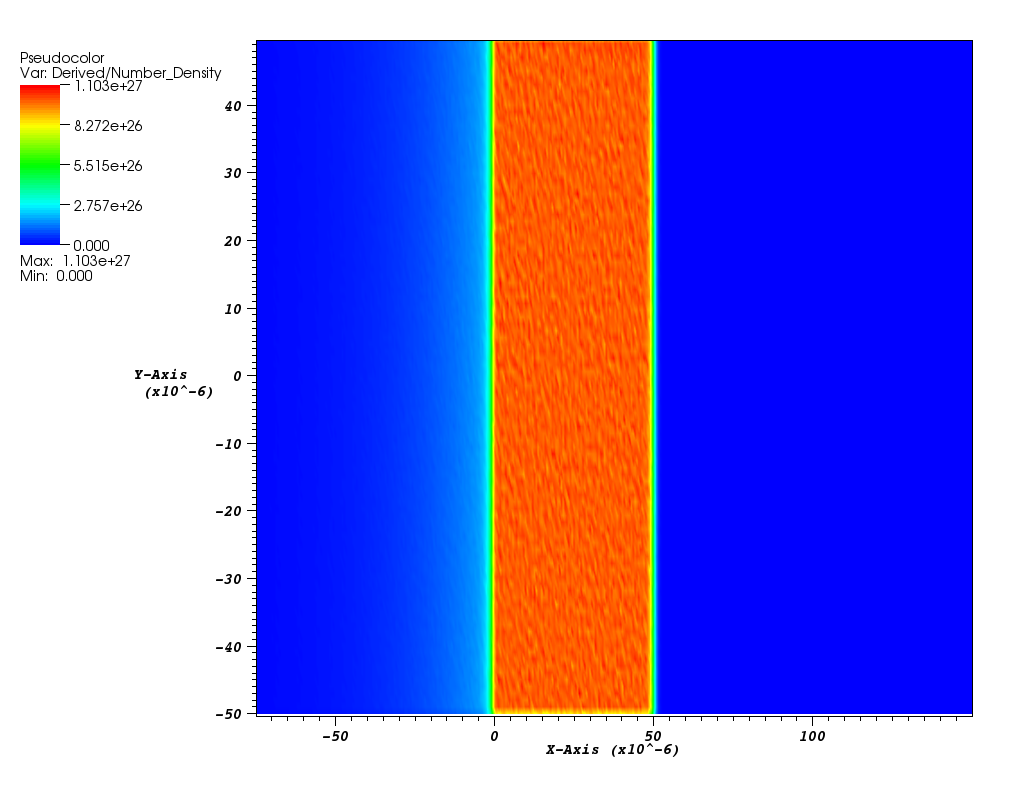
\includegraphics[width=0.8\linewidth]{images/visit_contour}
  \end{center}

  There are many settings which can alter the visual appearance
  of plots generated by VisIt. The first point of call is usually to
  open up the \qm{Plot Attributes} or \qm{Operator Attributes} dialogue
  corresponding to the
  plot in question. A simpler method for accomplishing this task is
  to double-click on the plot in the main VisIt menu pane which will
  launch the corresponding \qm{Plot Attributes} dialogue.

  If it is the operator attributes you wish to change,
  click on the white arrow on the left hand side of the plot in the
  main VisIt menu pane. This will drop down to reveal a list containing
  the plot and all operators acting on it. Double-clicking on an operator
  will launch the corresponding \qm{Operator Attributes} dialogue.
  \begin{center}
    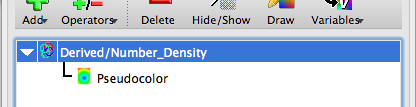
\includegraphics[width=0.7\linewidth]{images/visit_attrib}
  \end{center}

  Another important tool for controlling the appearance of plots can
  be found in \qm{Controls $\Rightarrow$ Annotation} from the VisIt menu
  bar. This allows all of the plot annotations to be modified such as
  the legend, title, axis labels, etc.
  \begin{center}
    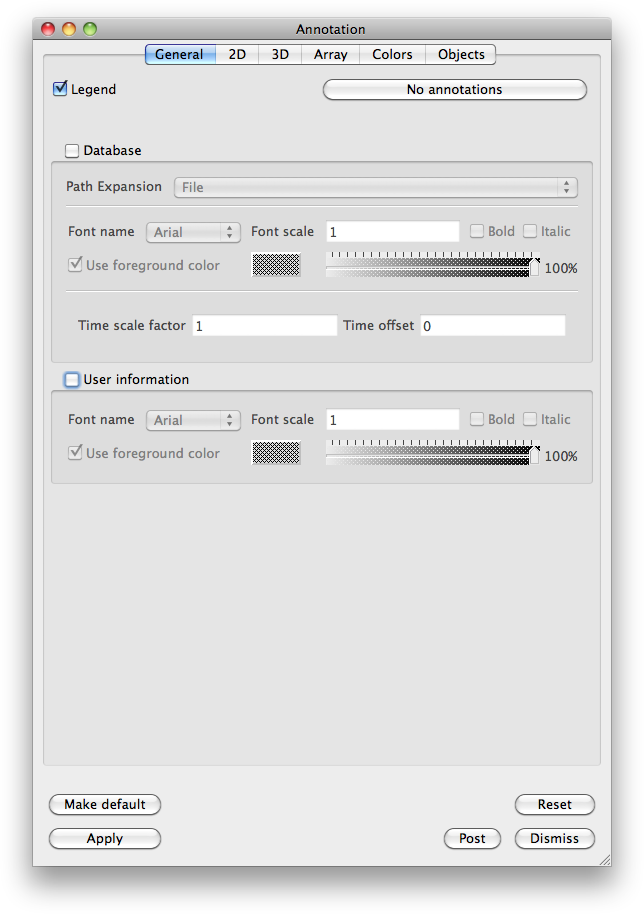
\includegraphics[width=0.6\linewidth]{images/visit_annot}
  \end{center}

\subsection{1D Plotting in VisIt}
  A 1D plot in VisIt is called a \qm{Curve} plot. We already mentioned that
  this was greyed out because we have no one dimensional variables in our
  data file.

  The solution to this dilemma is the lineout operator which extracts a
  one dimensional array from a 2D or 3D variable. This operator is selected
  by pressing the button with red and blue lines located at the top of
  the plot window.
  \begin{center}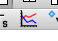
\includegraphics{images/visit_lineout}\end{center}

  Once the button has been pressed, we can click and drag anywhere in
  the \qm{Pseudocolor} plot window. When we release the mouse button a
  new plot window pops up containing a \qm{Curve} plot of the data just
  selected.
  \begin{center}
    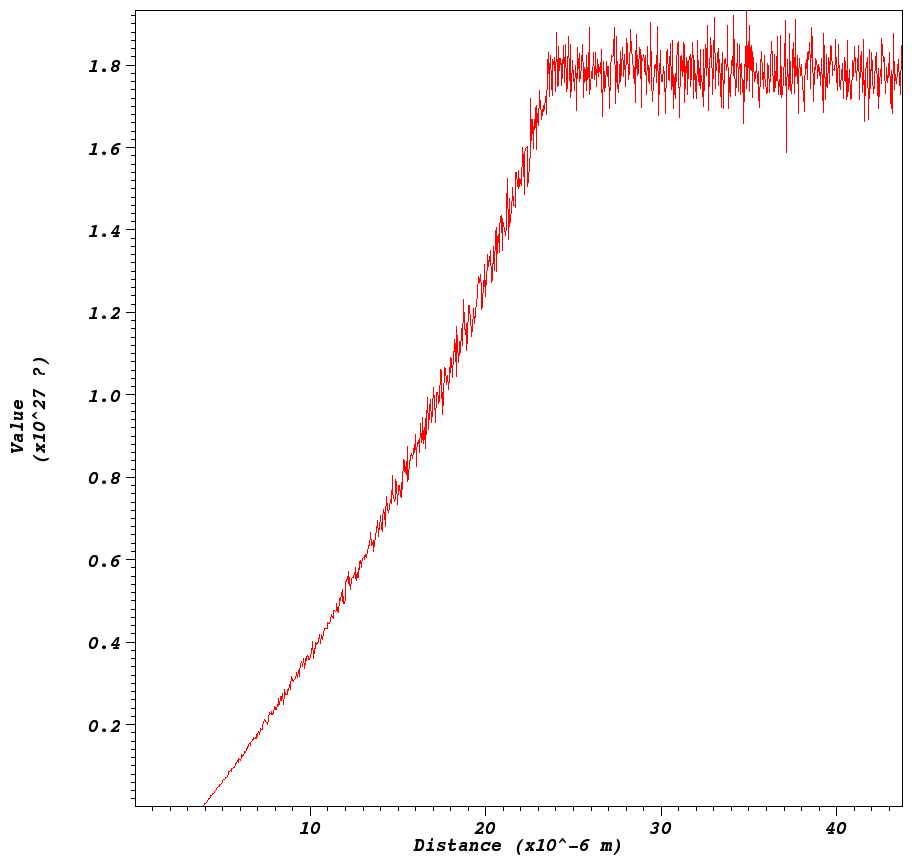
\includegraphics[width=0.8\linewidth]{images/visit_curve}
  \end{center}

  In order to change the attributes for this plot, we must first select
  \qm{Active window} number 2 in the main VisIt pane.

\subsection{Shaded Surface Plots in VisIt}
  Again, we will confusingly refuse to pick the obvious plot type for this
  task. There is \qm{Surface} plot listed in the menu. However, most of the
  time the \qm{Elevator} operator does what we want and also gives us more
  flexibility.

  The first step is to do a \qm{Pseudocolor} plot of \qm{Number\_Density} as
  we did before. Next select the \qm{OpAtts $\Rightarrow$ Elevate} menu item.
  In the pop up dialogue click on the \qm{Elevation height relative to XY
  limits} and then \qm{Apply}. Click \qm{Yes} when the warning dialogue pops
  up.
  \begin{center}
    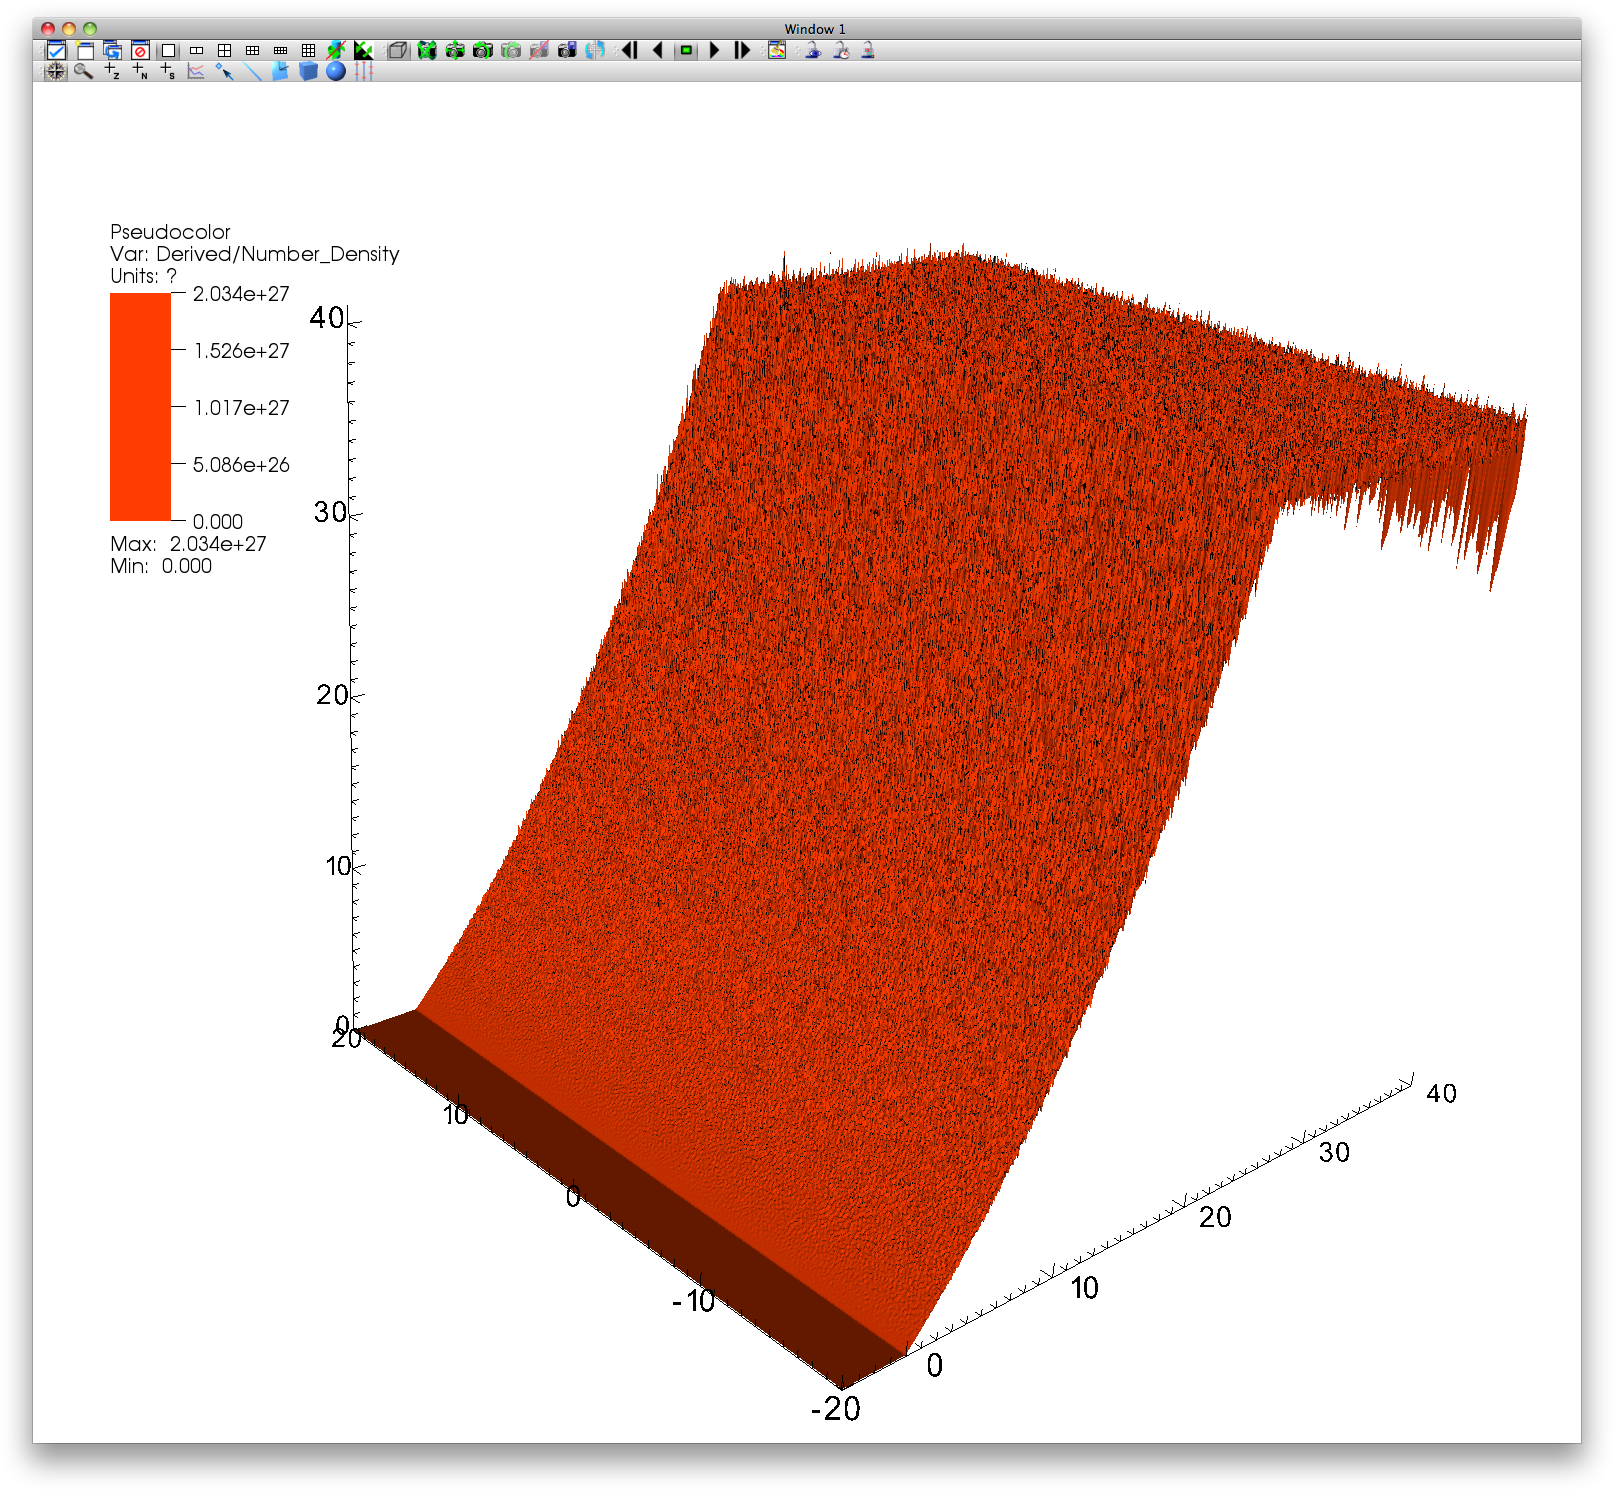
\includegraphics[width=0.8\linewidth]{images/visit_shade_surf}
  \end{center}

  To make this plot look similar to the one generated by IDL, we have changed
  the colour table using \qm{Controls $\Rightarrow$ Color table}.
  We also changed the axis appearance with the annotations menu discussed
  earlier and changed the height of the elevation using the min and max
  operator attributes.

\subsection{Creating User-Defined Expressions}
  VisIt comes with an extremely powerful method of manipulating data before
  visualising the results. The basic idea is that an array is transformed
  by applying a set of mathematical functions on all its elements and then
  the result is defined as a new variable. Once defined, this variable
  behaves in exactly the same way as any of the variables read from the
  data file.

  As an example, we can combine the three components of electric field
  to generate a single electric field vector.
  \begin{center}
    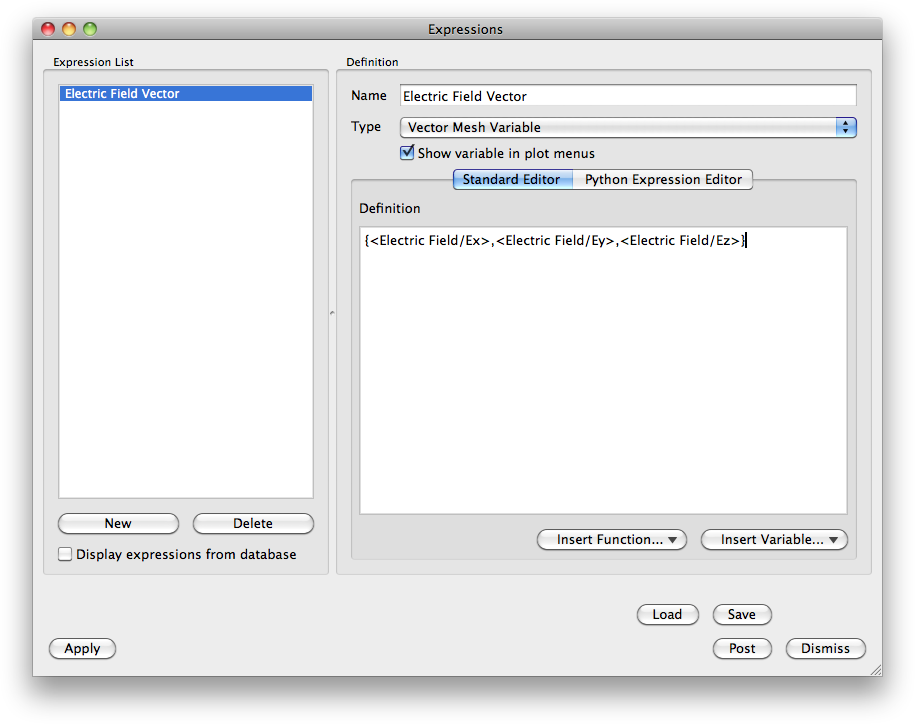
\includegraphics[width=0.8\linewidth]{images/visit_expression_vector}
  \end{center}

  Now when we return to the \qm{Add} menu we see that the \qm{Vector}
  and \qm{Streamline} plot types now have an entry for our newly defined
  vector.

\subsection{Creating Movies}
  A compelling visualisation of numerically generated data is often made
  by combining a series of images into a movie. This can be an invaluable
  method for illustrating the basic behaviour of a system as it changes
  over time. Alternatively rotating around a 3D scene can sometimes
  give a much better idea of the structure in the model being presented. 
  There can also be much to gain by constructing visual fly-throughs
  of a scene, dynamically slicing through sets of data or combinations
  of all these techniques.

  VisIt provides several facilities for generating movies from your
  data. The simplest of these is to select the \qm{File $\Rightarrow$
  Save movie} menu item. This pops up a movie wizard which will walk
  you through the process of generating a simple linear movie based
  on the time-advancing snapshots represented by your virtual database
  of files. Alternatively you can select one of the pre-defined movie
  templates which manipulate the currently selected plot and create
  a movie from that.

  Creating a simple time advancing movie is as simple as walking through
  the wizard dialogue and selecting from the self-explanatory options
  presented to you.

  For many uses, the wizard will give exactly the desired results. However
  it is occasionally useful to have a little more control over how the
  movie is created. In such cases it can be useful to specify an image
  format such as \qm{PNG} to save to rather than \qm{MPEG}. VisIt will
  then generate one image per frame and number them consecutively. At
  the end of the process the images can be converted into a movie using
  whatever tool best accomplishes the task.

  \begin{center}
    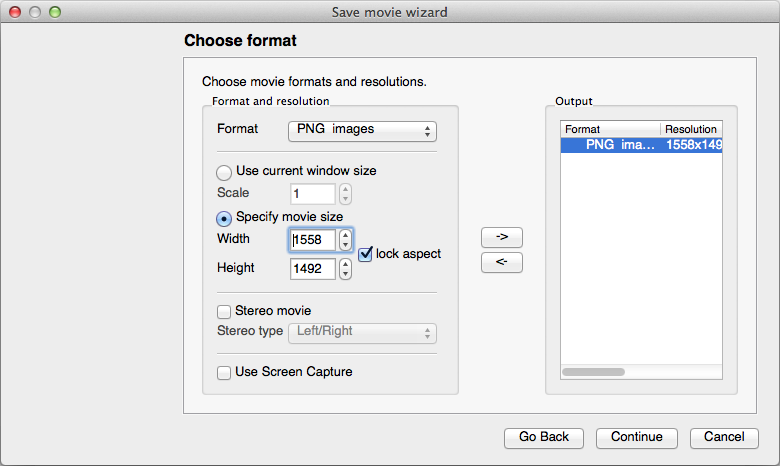
\includegraphics[width=0.8\linewidth]{images/visit_movie}
  \end{center}
  Another useful tip is to select the \qm{Later, tell me the command to
  run} radio button. This will output a long command which can run from
  a UNIX terminal screen. The advantage is that no X session is required
  so the command can be run in the background. It also becomes a simple
  task to interrupt the job at any point and resume it from where it
  left off at a later date. In a similar manner it is easy to resume
  a job which crashes half way through for any reason.

  More complex movies can be created by using VisIt's keyframing facility
  which allows you to change animation attributes such as view or plot
  attributes as the animation progresses. Further information about this
  somewhat complex task can be found in the on-line help.

  Finally, you can use VisIt's python scripting interface to programmatically
  describe the details of each frame as the movie progresses. This approach
  offers far more flexibility in what can be achieved but is also much
  more involved and time consuming than the previous two methods. Again,
  further information on this subject can be found in the on-line help
  system.

\subsection{Remote Visualisation}
  It was mentioned earlier that it is possible to perform remote visualisation
  using VisIt. This is a process in which the data files being interrogated
  reside on a different machine to the one on which the VisIt GUI runs and
  where the results are plotted.

  This method of working can be extremely useful when the data is generated
  on a powerful machine located in an external environment such as a large
  cluster. Another common use is when {\EPOCH} is executed on a UNIX machine
  and the desktop used for visualisation is running Windows.

  It is sometimes possible to run a graphical tool on the remote machine
  and tunnel the X-server session through to the local machine but this
  can be quite slow and unstable. When connecting to a remote VisIt
  instance the only data which needs to be sent between machines is the
  pre-rendered image and a few simple plotting commands. Naturally, this
  can be a {\em much} faster approach.

  Also, as mentioned before, it is possible to use a machine on which the
  reader plugin is difficult or impossible to compile for and connect
  to a machine on which the reader is already installed.

  In order to use the remote visualisation facility, you must first
  set up a \qm{Host Profile} for the remote machine using the \qm{Options
  $\Rightarrow$ Host Profiles} menu item. The pre-compiled binaries are
  shipped with a long list of pre-defined host profiles. These are unnecessary
  for anyone not affiliated and can safely be removed by deleting the
  directory \txt{\$HOME/visit/current/.visit/} (assuming you have unpacked
  the VisIt tarball into your home directory).

  \begin{center}
    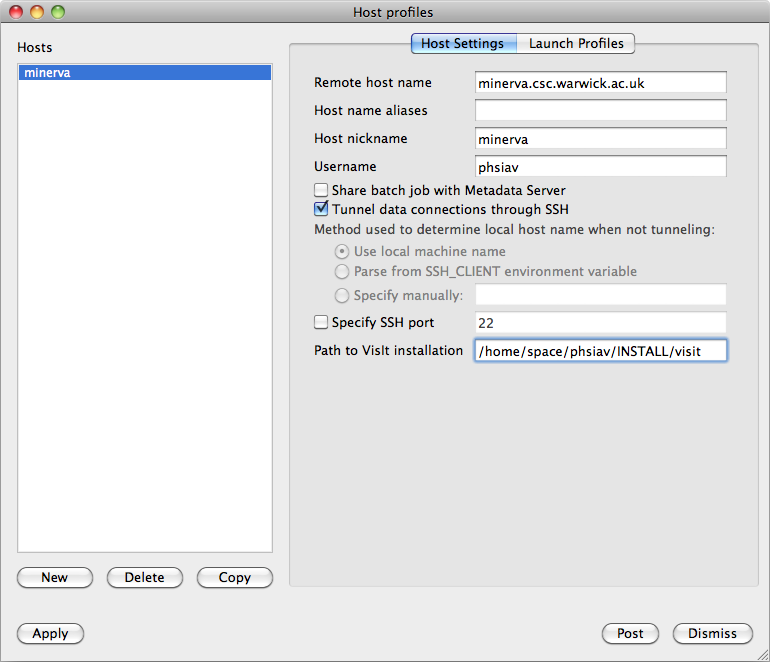
\includegraphics[width=0.8\linewidth]{images/visit_host_profile}
  \end{center}

  Create a new profile by clicking on the \qm{New profile} button and filling
  out some of the form fields. The important ones to change are \qm{Profile
  name}, \qm{Remote host name}, \qm{Host name aliases} and \qm{Username}.
  If the visit binary is not in your default search path on the remote
  machine then you must specify its location by passing \qm{-dir
  /base/installpath/visit} to \qm{Additional options}.

  Now select the \qm{Options $\Rightarrow$ Save Settings} menu item to
  ensure that the profile is saved for future sessions.

  Data on the remote machine can now be loaded by selecting \qm{File
  $\Rightarrow$ Open file} and picking the desired host profile
  from the drop down list of \qm{Hosts}. VisIt will wait for the
  remote process to launch and then continue with the file selection
  procedure but now displaying files located on the remote machine
  rather than the local one. From this point on everything should work
  as before except you should see the name of the remote machine in the
  \qm{Selected files} dialogue. 

  \begin{center}
    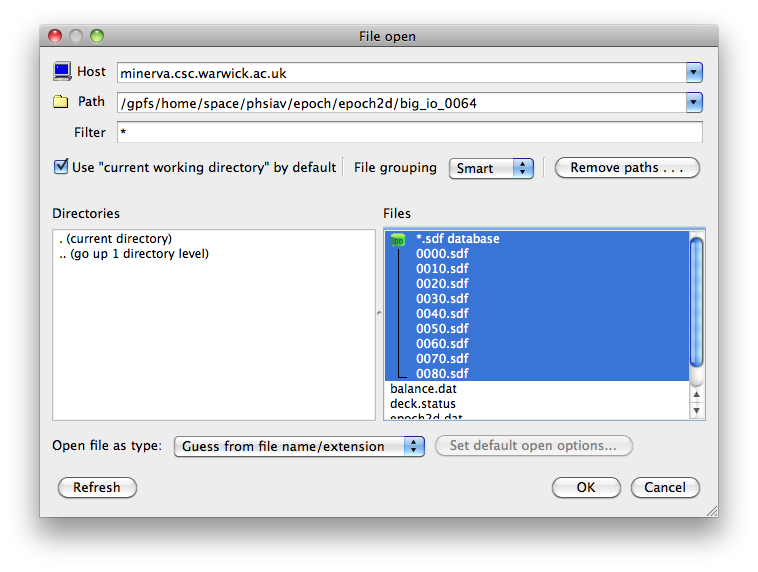
\includegraphics[width=0.8\linewidth]{images/visit_host_files}
  \end{center}

\subsection{Parallel Visualisation}
  Before reading this section be warned that the current version of
  the SDF reader is not capable of reading data in parallel! However,
  this is high on the list of issues to be addressed so a parallel
  version ought to be released some time in the near future.

  Parallel visualisation is performed in almost exactly the same manner
  as remote visualisation. Again, you must create a host profile for the
  purpose except this time you need to check the \qm{Parallel computation
  engine} radio button. This will activate a \qm{Parallel options} tab
  which must be filled in to match the cluster on which the job will
  be launched.

  The major difference now is due to the fact that VisIt must be launched
  by an external job script which fits in with the queueing system used
  by the parallel machine. Usually you will need to consult with the
  system administrator of the cluster to confirm which launch method and
  arguments to use.

  The details of job launch can be better understood by reading through
  the file\linebreak \txt{\$HOME/visit/current/bin/internallauncher}. This is
  a bash script which parses the arguments and executes the specified
  launch method.
%\subsection{Examples}
%  \begin{itemize}
%  \item
%  \end{itemize}
%\section*{Summary}
%
%\begin{frame}{Summary}
%
%  % Keep the summary *very short*.
%  \begin{itemize}
%  \item
%    Item 1
%  \end{itemize}
%\end{frame}

